% This file was adapted from ICLR2022_conference.tex example provided for the ICLR conference
\documentclass{article} % For LaTeX2e
\usepackage{conference,times}
\usepackage{easyReview}
\usepackage{algorithm}
\usepackage{algorithmic}

% Optional math commands from https://github.com/goodfeli/dlbook_notation.
\input{math_commands.tex}

\usepackage{amsthm,amssymb}

\newtheorem{theorem}{Theorem}[section]
\newtheorem{corollary}{Corollary}[theorem]
\newtheorem{lemma}[theorem]{Lemma}
\newtheorem{definition}[theorem]{Definition}

% Please leave these options as they are
\usepackage{hyperref}
\hypersetup{
    colorlinks=true,
    linkcolor=red,
    filecolor=magenta,
    urlcolor=blue,
    citecolor=purple,
    pdftitle={Parity-Locked Quantum Reservoir Computing for PCA-Encoded Image Classification},
    pdfpagemode=FullScreen,
    }



\title{Parity-Locked Quantum Reservoir Computing for PCA-Encoded Image Classification:\\
Robust Advantage, Entanglement Frontiers, and Operator--Dynamics Attribution}

\author{Anonymous Authors \\
Affiliation withheld for review \\
\texttt{anonymous@domain.edu}}

\begin{document}


\maketitle

\begin{abstract}
Quantum reservoir computing for image classification is currently constrained by a reproducibility problem: many reported improvements can be explained by uneven preprocessing, readout mismatch, or benchmark saturation rather than by reservoir physics. We study this issue in a parity-locked protocol where quantum and classical reservoirs share fold-local PCA, feature budget, readout family, tuning budget, and split seeds, and where a transverse-Ising reservoir is evaluated with matched entangling and non-entangling branches. We formalize three audit quantities: a robust non-easy-tier gap functional $\Delta_{\mathrm{rob}}$, a matched-control entanglement effect $\tau(\eta,S)$ over noise-shot strata, and an attribution ratio $\rho(\eta)$ that separates observable-policy gains from dynamics gains with an explicit undefined-denominator guard. Symbolic checks verify the algebraic identities used by the audit quantities, including gap-error equivalence and ratio-domain conditions. Simulation evidence on tiered image regimes shows positive robust gaps on mid and hard tiers under protocol parity, regime-dependent entanglement effects with unresolved cells at high noise and low shots, and mixed operator-vs-dynamics dominance because ratio estimates become undefined near small dynamics denominators. The resulting conclusion is conditional rather than universal: parity-controlled quantum advantage is supported in identified robustness regimes, but attribution and frontier claims require explicit caveats where uncertainty or denominator instability dominates.
\end{abstract}

\section{Introduction}
\label{sec:intro}
Quantum reservoir computing (QRC) has become a central candidate for resource-limited quantum machine learning because it separates fixed nonlinear dynamics from a lightweight classical readout, a design philosophy that mirrors classical reservoir computing and echo-state models \citep{url_echo_state_2001,doi_10_1162_089976602760407955,arxiv_2102_11831}. In image settings, this framework is often instantiated by encoding a low-dimensional feature vector into a qubit circuit, evolving under a fixed Hamiltonian, and extracting observables that feed a linear or kernelized predictor \citep{arxiv_2409_00998,arxiv_2602_14677,arxiv_2602_18377}. The current literature nevertheless remains contradictory on whether measured gains are due to genuinely quantum reservoir dynamics, to expressive encoding maps that would also benefit non-reservoir models, or to measurement operator tuning that can dominate any dynamics effect \citep{arxiv_2101_11020,arxiv_2008_08605,arxiv_2503_17939,arxiv_2503_22380,arxiv_2602_17440}.

The practical implication is immediate for the user-facing question of this study: does a PCA-encoded quantum reservoir outperform matched classical reservoirs on image classification, and what is the role of entanglement in that comparison? Without strict protocol parity, the answer is not scientifically identifiable. If one branch uses different PCA fitting scope, readout capacity, hyperparameter search budget, or split seeds, then observed differences cannot be attributed to reservoir physics. If evaluation is restricted to easy datasets, separability ceilings can mask both true positives and true negatives \citep{arxiv_2212_08693,arxiv_2412_06758,arxiv_2601_22194}. If uncertainty is ignored in noisy, finite-shot settings, claims about entanglement can flip sign under realistic channel assumptions \citep{arxiv_2403_08998,arxiv_2209_05142,arxiv_2509_06873,arxiv_2601_23084}.

This paper treats these concerns as first-class methodological constraints rather than post-hoc checks. We construct a parity-locked hybrid analysis that combines formal claim audits with simulation evidence. The formal component defines and proves identities required to interpret robust advantage and attribution quantities. The simulation component evaluates tiered image regimes under matched controls and quantifies where support is strong, mixed, or unresolved. The objective is not to maximize one headline metric, but to establish a defensible claim boundary: what can be supported under the executed protocol, what is conditional, and what remains unresolved.

Our introduction-level contributions are the following.
\begin{itemize}
\item We define a parity-feasible comparison space for quantum and classical reservoirs and formalize a robust non-easy-tier advantage quantity $\Delta_{\mathrm{rob}}$ that prevents easy-tier saturation from dominating conclusions.
\item We introduce a matched-control entanglement estimand $\tau(\eta,S)$ and a sign-frontier interpretation over noise-shot strata, explicitly separating supported and unresolved regions.
\item We formalize an operator--dynamics attribution ratio $\rho(\eta)$ with an explicit denominator-domain guard, so ratio claims cannot be made where dynamics effects are numerically unstable.
\item We connect each major claim to executable evidence (figures, tables, symbolic checks, and falsification diagnostics), making negative or mixed outcomes part of the main narrative rather than relegated to omitted notes.
\end{itemize}

Beyond the immediate QRC setting, the broader relevance is methodological: parity-audited comparison protocols are necessary whenever hybrid quantum-classical studies involve expressive encodings, high-variance estimators, and optimization-heavy measurement policies. The same audit logic applies to kernelized quantum models, analog reservoirs, and measurement-feedback systems \citep{arxiv_2407_02553,arxiv_2310_06706,arxiv_2602_00610,arxiv_2602_19700,arxiv_2603_20167}. In that sense, our contribution is both domain-specific and transferable: specific to transverse-Ising image-QRC here, and transferable as an evaluation blueprint for nearby architectures.

\section{Related Work, Contradictions, and Novelty Boundary}
\label{sec:related}
\subsection{Classical Reservoir Foundations and Parity Requirements}
The foundational RC literature established the principle that fixed recurrent dynamics plus a trained readout can provide strong performance while keeping optimization manageable \citep{url_echo_state_2001,doi_10_1162_089976602760407955}. Later analyses emphasized that fair comparison requires matching state dimension, readout family, and training protocol, because small differences in these elements can dominate outcomes \citep{arxiv_2102_11831,arxiv_2201_07969}. We adopt this baseline logic directly: in this manuscript, parity is not a reporting preference but part of the feasible set that defines what counts as admissible evidence.

\subsection{Encoding Geometry and Kernel Explanations}
A major thread in quantum ML shows that supervised quantum models can often be interpreted through kernels and feature maps, implying that representational geometry can explain a substantial portion of observed performance \citep{arxiv_2101_11020,arxiv_2008_08605,arxiv_2502_06281,arxiv_2602_19644}. This perspective introduces an immediate caution for QRC image claims. If angle encoding and PCA already induce a strong geometry, architecture-level advantage may be overstated unless encoding and feature budgets are parity-matched across branches. Our method therefore treats encoding and measurement budgets as controlled factors, not hidden degrees of freedom.

\subsection{Entanglement as Utility vs Fragility}
The literature reports both positive and skeptical views on entanglement utility. Several studies show improved separability or classification behavior when entangling operations are present \citep{arxiv_2403_08998,arxiv_2209_05142,arxiv_2511_01387}. In contrast, recent analyses show that under local depolarizing noise, finite shots, and simulability constraints, apparent gains can attenuate or vanish \citep{arxiv_2509_06873,arxiv_2601_23084}. This contradiction is central to our work. We do not ask whether entanglement is globally beneficial; we ask where matched-control evidence supports a positive effect and where the frontier remains unresolved.

\subsection{Operator Optimization vs Reservoir Dynamics}
Recent QRC papers increasingly optimize measurement operators, Pauli subsets, or readout-facing quantum features \citep{arxiv_2602_14677,arxiv_2602_18377,arxiv_2602_17440}. In parallel, recurrence-focused studies argue that feedback and richer dynamics are primary \citep{arxiv_2503_17939,arxiv_2503_22380,arxiv_2601_04812}. These positions are not mutually exclusive, but they imply different mechanism claims. Our novelty boundary is to avoid collapsing them into one score: we define a ratio-based attribution quantity to test whether operator gains dominate dynamics gains under fixed budgets, and we explicitly mark bins where the ratio is undefined.

\subsection{Benchmark Hardness and Protocol Realism}
Image-QRC studies often use MNIST-like regimes because they are computationally accessible \citep{arxiv_2409_00998,arxiv_2212_08693}. However, multiple sources note that easy datasets with aggressive preprocessing can saturate, reducing interpretability of small accuracy differences \citep{arxiv_2412_06758,arxiv_2601_22194,arxiv_2512_11367,arxiv_2512_18612}. This motivates our tiered hardness framing and robust non-easy-tier functional. The novelty is not another benchmark list, but a claim policy: advantage claims are gated by non-easy tiers and uncertainty-aware criteria.

\subsection{Novelty Boundary Relative to Prior Work}
Our contribution sits at a defensible boundary defined by four elements. First, we unify parity constraints from classical RC baselines with quantum-specific controls over encoding, observables, noise, and shots. Second, we formalize and prove identities that are often used implicitly but not audited explicitly in QRC reports. Third, we attach each high-level claim to concrete evidence objects, including mixed outcomes and stress failures. Fourth, we treat unresolved regions as scientific outputs, not as missing polishing. This is distinct from purely benchmark-centric papers, purely mechanistic papers, or purely hardware demonstrations \citep{arxiv_2407_02553,arxiv_2310_06706,arxiv_2602_00610,arxiv_2603_17182,arxiv_2602_21544,arxiv_2602_13094}.


\subsection{Comparison Matrix Synthesis}
To make the novelty boundary operational, we summarize the literature along five recurring axes and connect each axis to an explicit risk of overclaiming. The first axis is \emph{source of gains}: reservoir dynamics versus measurement policy. Studies focused on operator optimization show that careful observable selection can deliver large improvements without changing recurrent dynamics \citep{arxiv_2602_14677,arxiv_2602_18377}. In contrast, recurrence- and feedback-oriented studies attribute gains to richer temporal state evolution \citep{arxiv_2503_17939,arxiv_2503_22380,arxiv_2602_17440}. Our response is to estimate both effects and to avoid single-cause narratives when denominator stability is weak.

The second axis is \emph{entanglement utility under noise}. Positive findings are often reported in controlled settings with favorable noise and measurement budgets \citep{arxiv_2403_08998,arxiv_2209_05142}. Skeptical results appear when local depolarization, finite shots, and simulability constraints are modeled aggressively \citep{arxiv_2509_06873,arxiv_2601_23084}. We therefore formulate entanglement conclusions as frontier statements indexed by $(\eta,S)$ rather than as globally signed outcomes.

The third axis is \emph{benchmark hardness}. Papers that emphasize easy image regimes can report competitive performance, but disagreement rises when hardness, domain shift, or stronger classical baselines are introduced \citep{arxiv_2409_00998,arxiv_2212_08693,arxiv_2412_06758,arxiv_2601_22194}. Our robust objective explicitly excludes easy-tier dominance to reduce this source of disagreement.

The fourth axis is \emph{encoding expressivity versus architecture novelty}. Kernel-based analyses demonstrate that expressive embeddings can dominate model behavior even when downstream training is simple \citep{arxiv_2101_11020,arxiv_2008_08605,arxiv_2502_06281}. We therefore treat encoding and measurement budgets as controlled factors and avoid attributing all observed gains to reservoir dynamics.

The fifth axis is \emph{platform transfer}. Analog hardware and Rydberg demonstrations show promising scalability trends, but calibration overhead, device-specific channel behavior, and measurement costs complicate direct comparison with simulator-first pipelines \citep{arxiv_2407_02553,arxiv_2310_06706,arxiv_2602_00610}. This axis motivates our explicit limitation statements and the follow-up hardware calibration plan.

\section{Problem Setting and Formal Scope}
\label{sec:problem}
\subsection{Data, Encodings, and Reservoir Families}
Let $\train=\{(x_i,y_i)\}_{i=1}^{n}$ denote labeled examples and let $d\in\{D_{\mathrm{easy}},D_{\mathrm{mid}},D_{\mathrm{hard}}\}$ index benchmark hardness tiers. For each fold $k$, we fit a PCA map $P_k:\mathbb{R}^{p}\to\mathbb{R}^{r}$ on training examples only, and define $z_i=P_k(x_i)$. This fold-local requirement is part of the feasible protocol; violating it is a leakage event.

The quantum branch uses angle encoding $U_{\mathrm{enc}}(z)$ on $n_q$ qubits, followed by transverse-Ising reservoir evolution with control parameters $\Theta=(J,h,\text{depth})$ and optional entangling terms indicated by $e\in\{0,1\}$. Measured observables form a set $\mathcal{O}=\{O_j\}_{j=1}^{m}$, and features are
\begin{equation}
\label{eq:q_feature}
f_q(x)=\big(\operatorname{Tr}(O_1\rho(x)),\ldots,\operatorname{Tr}(O_m\rho(x))\big),
\end{equation}
where $\rho(x)$ is the post-evolution state.

The classical branch uses matched dimensionality $m$ and the same readout family. We denote its features by $f_c(x)\in\mathbb{R}^{m}$. Both branches use the same linear-ridge readout class, the same search budget $B$, and the same split seeds. These controls encode baseline parity inherited from RC practice \citep{url_echo_state_2001,doi_10_1162_089976602760407955}.

\subsection{Decision Variables, Feasible Set, and Objective}
We optimize model selection inside a parity-feasible set $\mathcal{F}$:
\begin{equation}
\label{eq:feasible_set}
\mathcal{F}=\left\{\theta:\;m_q=m_c,\;\mathcal{H}_{\mathrm{readout}}^q=\mathcal{H}_{\mathrm{readout}}^c,\;B_q=B_c,\;P_k \text{ fit on train only},\;\Xi_q=\Xi_c\right\},
\end{equation}
where $\Xi$ denotes the shared noise-shot grid over depolarizing rate $\eta$ and shot count $S$.

Define per-tier gap
\begin{equation}
\label{eq:gap}
g_d(\eta,S;\theta)=A_q(d,\eta,S;\theta)-A_c(d,\eta,S;\theta),
\end{equation}
and robust objective
\begin{equation}
\label{eq:robust_obj}
\Delta_{\mathrm{rob}}(\theta)=\min_{d\in\{D_{\mathrm{mid}},D_{\mathrm{hard}}\}}\mathbb{E}_{(\eta,S)\sim\Pi}\left[g_d(\eta,S;\theta)\right].
\end{equation}
The primary decision variable is $\theta\in\mathcal{F}$, including encoding depth, observable subset, and regularization settings subject to parity constraints. The primary optimality criterion is
\begin{equation}
\label{eq:argmax}
\theta^{\star}\in\arg\max_{\theta\in\mathcal{F}}\Delta_{\mathrm{rob}}(\theta).
\end{equation}
This objective is intentionally non-easy-tier; it operationalizes the requirement that main claims should survive beyond saturation-prone settings.

\subsection{Manuscript-Specific Audit Quantities}
In this work we define two additional quantities to resolve literature contradictions.
First, for entanglement treatment $e\in\{0,1\}$ and loss $L=1-A$, we define
\begin{equation}
\label{eq:tau}
\tau(d,\eta,S,\ell)=\mathbb{E}[L\mid e=0,d,\eta,S,\ell]-\mathbb{E}[L\mid e=1,d,\eta,S,\ell],
\end{equation}
where $\ell$ indexes observable policy. Positive $\tau$ means entanglement reduces loss.

Second, to separate operator from dynamics effects we define
\begin{equation}
\label{eq:rho}
\rho(\eta)=\frac{\Delta A_{\mathrm{obs}}(\eta)}{\Delta A_{\mathrm{dyn}}(\eta)},
\end{equation}
with the domain guard $|\Delta A_{\mathrm{dyn}}(\eta)|>\varepsilon$. If the denominator guard fails, $\rho$ is undefined and no dominance claim is admissible.

Borrowed components are explicitly sourced: kernel-view feature geometry \citep{arxiv_2101_11020,arxiv_2008_08605}, entanglement/noise caveats \citep{arxiv_2509_06873,arxiv_2601_23084}, and operator optimization framing \citep{arxiv_2602_14677,arxiv_2602_18377}. The robust objective and ratio-domain claim policy are introduced in this manuscript.


\subsection{Assumption Ledger and Provenance Discipline}
Our problem formulation uses a mixed provenance model: some quantities are inherited from prior literature, while others are introduced specifically for this manuscript. The inherited components include feature-map interpretation for encoded quantum models \citep{arxiv_2101_11020,arxiv_2008_08605}, fixed-reservoir baseline logic \citep{url_echo_state_2001,doi_10_1162_089976602760407955}, and noise-aware entanglement caveats \citep{arxiv_2509_06873,arxiv_2601_23084}. The manuscript-specific components are the robust non-easy-tier objective gate, the sign-frontier presentation policy for $\tau$, and the denominator-guard policy for $\rho$.

We make this distinction explicit because ambiguity between sourced conventions and manuscript-defined audit rules is a common source of reproducibility failures. If a reader cannot identify which assumptions are inherited and which are newly imposed, result interpretation becomes fragile across reruns. In our setting, reproducibility requires that parity assumptions be treated as hard constraints, not tunable options.

The practical ledger is as follows. \emph{Data assumptions}: fold-local PCA and fixed tier labels. \emph{Model assumptions}: matched readout class and matched optimization budget. \emph{Measurement assumptions}: fixed observable budget and explicit treatment of optimized versus canonical policies. \emph{Noise assumptions}: shared $(\eta,S)$ grid and explicit unresolved-cell reporting under confidence overlap. \emph{Attribution assumptions}: denominator positivity for ratio claims. If any ledger item fails, associated claim status is downgraded by construction.

\section{Methodology: Hybrid Formal and Simulation Audit}
\label{sec:method}
\subsection{Parity-Audit Protocol}
Our methodology combines three modules: (i) parity validation, (ii) theorem-backed quantity interpretation, and (iii) uncertainty-aware simulation diagnostics. The parity module checks fold-local PCA, matched feature/readout budgets, and shared split seeds before any ranking. The formal module proves identities needed to interpret the reported quantities. The simulation module computes bootstrap confidence intervals and records unresolved regions when support is insufficient.

This structure is designed to prevent methodological shortcuts. For example, if parity checks fail, a positive gap is not interpreted as evidence for reservoir advantage. If denominator stability fails for \eqref{eq:rho}, ratio dominance is explicitly withheld. If a confidence interval straddles zero on the entanglement frontier, the corresponding cell is unresolved rather than forced into a binary decision.

\subsection{Formal Statements and Proofs}
\begin{definition}[Parity-locked robust advantage]
\label{def:delta_rob}
Given $\theta\in\mathcal{F}$, we call $\Delta_{\mathrm{rob}}(\theta)$ from \eqref{eq:robust_obj} the parity-locked robust advantage functional. A conditional advantage claim is admissible only if an estimated lower confidence bound for $\Delta_{\mathrm{rob}}$ is strictly positive.
\end{definition}

\begin{lemma}[Gap-error equivalence]
\label{lem:gap_error}
Let $E_b=1-A_b$ for branch $b\in\{q,c\}$. Then
\begin{equation}
\label{eq:gap_error_identity}
(E_c-E_q)-(A_q-A_c)=0.
\end{equation}
\end{lemma}
\begin{proof}
By substitution, $E_c-E_q=(1-A_c)-(1-A_q)=A_q-A_c$. Rearranging gives \eqref{eq:gap_error_identity}. This identity is exact and does not rely on distributional assumptions.
\end{proof}

\begin{theorem}[Lower-bound transfer for robust advantage]
\label{thm:delta_rob_lb}
Suppose there exists $\gamma\in\mathbb{R}$ such that for each $d\in\{D_{\mathrm{mid}},D_{\mathrm{hard}}\}$,
\begin{equation}
\label{eq:lb_assumption}
\mathbb{E}_{(\eta,S)\sim\Pi}[g_d(\eta,S;\theta)]\ge \gamma.
\end{equation}
Then $\Delta_{\mathrm{rob}}(\theta)\ge \gamma$.
\end{theorem}
\begin{proof}
By definition, $\Delta_{\mathrm{rob}}(\theta)=\min\{u_{\mathrm{mid}},u_{\mathrm{hard}}\}$ where $u_d=\mathbb{E}_{(\eta,S)\sim\Pi}[g_d(\eta,S;\theta)]$. Under \eqref{eq:lb_assumption}, both $u_{\mathrm{mid}}$ and $u_{\mathrm{hard}}$ are at least $\gamma$. The minimum of two numbers each bounded below by $\gamma$ is also bounded below by $\gamma$. Hence $\Delta_{\mathrm{rob}}(\theta)\ge\gamma$.
\end{proof}

\begin{definition}[Matched-control entanglement effect]
\label{def:tau}
For strata $(d,\eta,S,\ell)$ that satisfy consistency, exchangeability, and positivity, we define the entanglement effect $\tau$ by \eqref{eq:tau}. Positive values indicate lower loss under entangling dynamics.
\end{definition}

\begin{lemma}[Loss-accuracy form equivalence]
\label{lem:tau_equiv}
Under $L=1-A$,
\begin{equation}
\label{eq:tau_equiv}
\tau(d,\eta,S,\ell)=\mathbb{E}[A\mid e=1,d,\eta,S,\ell]-\mathbb{E}[A\mid e=0,d,\eta,S,\ell].
\end{equation}
\end{lemma}
\begin{proof}
Substitute $L=1-A$ into \eqref{eq:tau}: 
\(\tau=\mathbb{E}[1-A\mid e=0]-\mathbb{E}[1-A\mid e=1]=\mathbb{E}[A\mid e=1]-\mathbb{E}[A\mid e=0]\), which proves \eqref{eq:tau_equiv}.
\end{proof}

\begin{definition}[Operator--dynamics attribution ratio with guard]
\label{def:rho_guarded}
For noise level $\eta$, define $\rho(\eta)$ by \eqref{eq:rho} when $|\Delta A_{\mathrm{dyn}}(\eta)|>\varepsilon$. If $|\Delta A_{\mathrm{dyn}}(\eta)|\le\varepsilon$, $\rho(\eta)$ is undefined and excluded from dominance inference.
\end{definition}

\begin{lemma}[Dominance equivalence under positive denominator]
\label{lem:rho_dom}
If $\Delta A_{\mathrm{dyn}}(\eta)>0$, then
\begin{equation}
\label{eq:rho_dom}
\rho(\eta)>1 \iff \Delta A_{\mathrm{obs}}(\eta)>\Delta A_{\mathrm{dyn}}(\eta).
\end{equation}
\end{lemma}
\begin{proof}
With positive denominator, multiplying inequalities by $\Delta A_{\mathrm{dyn}}(\eta)$ preserves order:
\(\rho(\eta)>1\iff \Delta A_{\mathrm{obs}}(\eta)/\Delta A_{\mathrm{dyn}}(\eta)>1\iff \Delta A_{\mathrm{obs}}(\eta)>\Delta A_{\mathrm{dyn}}(\eta)\).
If denominator positivity is not satisfied, the implication is not admissible, which motivates Definition~\ref{def:rho_guarded}.
\end{proof}

\subsection{Claim-Audit Workflow}
\begin{algorithm}[t]
\caption{Parity-Locked Claim Audit Workflow}
\label{alg:audit}
\begin{algorithmic}[1]
\STATE Build fold-local PCA features and matched train/validation/test splits for all model families.
\STATE Enforce parity constraints from \eqref{eq:feasible_set}; if any constraint fails, mark the cell as inadmissible.
\STATE Compute $\Delta_{\mathrm{rob}}$ via \eqref{eq:robust_obj}, $\tau$ via \eqref{eq:tau}, and guarded $\rho$ via \eqref{eq:rho}.
\STATE Run symbolic identities from \eqref{eq:gap_error_identity}, \eqref{eq:tau_equiv}, and \eqref{eq:rho_dom} with denominator guard checks.
\STATE Estimate uncertainty using stratified bootstrap over seeds/folds/noise-shot cells.
\STATE Assign support labels: supported, mixed, or unresolved, and register falsification outcomes.
\end{algorithmic}
\end{algorithm}

\Algref{alg:audit} links formal statements to executable decisions. The algorithm is intentionally conservative: unresolved strata are preserved in the evidence map instead of being averaged away. This design follows the contradiction-aware intent of the study and avoids overstating global claims.


\subsection{Architecture and Module Responsibilities}
Although the contribution is centered on audit formalization, the computational pipeline has a clear module structure that matters for interpretation. The \emph{encoding module} maps fold-local PCA outputs into angle-encoded qubit states and corresponding classical parity features. The \emph{reservoir module} applies either entangling or non-entangling transverse-Ising evolution under matched depth and control schedules. The \emph{measurement module} produces fixed-budget observable summaries under canonical or optimized policies. The \emph{readout module} trains matched linear-ridge predictors under identical search budgets. The \emph{audit module} performs parity checks, symbolic checks, uncertainty estimation, and claim labeling.

These responsibilities are intentionally separated so that mechanism claims can be traced to the module where changes occur. For example, a gain achieved by switching from canonical to optimized observables is assigned to the measurement module, not to reservoir dynamics. Likewise, a gain that disappears after fold-local PCA correction is assigned to preprocessing leakage rather than to quantum dynamics. This modular accounting is essential to avoid mechanism conflation.

From a systems perspective, this architecture mirrors strong practice in hybrid scientific software: separate state evolution, feature extraction, and statistical interpretation so each can be validated independently. The symbolic-check module in particular acts as a bridge between formal statements and simulation outputs, ensuring that algebraic identities used in text are actively validated rather than assumed.

\section{Experimental Protocol and Reproducibility Setup}
\label{sec:protocol}
\subsection{Tiered Data Regimes and Baselines}
The protocol uses three tier labels ($D_{\mathrm{easy}},D_{\mathrm{mid}},D_{\mathrm{hard}}$) with five seeds $\{7,11,19,23,42\}$, noise levels up to $\eta=0.02$, and shot counts between 64 and 8192 depending on sub-study. The baseline family includes entangling and non-entangling QRC branches, classical echo-state and random-feature baselines, RBF-kernel SVM, and a quantum-kernel no-reservoir comparator. This breadth is required by the literature contradiction map: without both classical and quantum non-reservoir comparators, attribution claims are incomplete \citep{arxiv_2409_00998,arxiv_2602_14677,arxiv_2101_11020,arxiv_2212_08693}.

The design also includes stress controls for label shuffle and intentional leakage, not as auxiliary extras but as active falsification probes. These probes test whether the audit protocol can detect artificial gains. A methodology that cannot detect leakage inflation cannot credibly claim robustness.

\subsection{Noise, Shots, and Uncertainty}
Noise is modeled through depolarizing channels indexed by $\eta$, and finite-shot measurement uncertainty is represented by shot count $S$. For robust gap and frontier quantities, we use bootstrap confidence intervals across seeds and strata, consistent with simulation budget constraints. For operator-attribution ratios, undefined bins are explicitly tracked when denominator magnitude falls below tolerance.

The uncertainty policy is central for interpretation. In this manuscript, an unresolved confidence region is evidence of limited identifiability, not a failure to post-process data. This is especially important for entanglement frontiers and ratio-crossing claims, where sign decisions can be unstable in sparse high-noise cells \citep{arxiv_2509_06873,arxiv_2601_23084,arxiv_2602_00610}.

\subsection{Compute Budget and Repetition Design}
All experiments are executed under CPU-only constraints on Apple Silicon-class hardware, with staged runtime budgets across four simulation blocks. This constrained setting reflects the real operational envelope in which many QRC studies are run before hardware transfer. It also motivates careful sweep design: broad enough to test claim boundaries, but not so broad that uncertainty estimation becomes underpowered by exhausted compute.


Reproducibility relies on fixed seeds, pinned sweep grids, symbolic check reports, and exported tables and figures. The appendix documents all key settings, including sweeps over qubit counts, shot counts, PCA rank, noise levels, and observable budgets.

\subsection{Why Tiered Image Regimes Are Still Informative for Reservoir Analysis}
A common critique is that image tasks are less natural than sequence tasks for reservoir-style arguments. We agree that this is a legitimate concern, and we therefore avoid claiming direct equivalence between temporal-capacity theory and static image behavior. However, tiered image regimes remain informative for three reasons. First, they expose preprocessing sensitivity, which is central to parity auditing and independent of temporal semantics. Second, they allow controlled evaluation of entanglement and observable policies under fixed compute budgets. Third, they provide a reproducible bridge between classical RC fairness principles and quantum-specific measurement constraints.

The relevant distinction is not ``image versus sequence'' in the abstract, but whether the experimental object supports auditable claim closure. In this work, the auditable objects are robust non-easy-tier gaps, matched-control entanglement effects, and denominator-guarded attribution ratios. These objects can be evaluated in tiered image regimes without pretending that all sequence-theoretic quantities transfer unchanged. When transfer assumptions are not required, we do not introduce them. When we borrow concepts that originated in sequence settings, we explicitly bound their role to protocol design intuition rather than theorem-level dependence \citep{arxiv_2603_21371,arxiv_2602_21544,arxiv_2603_17182}.

This choice also aligns with the user-constrained compute envelope. Under CPU-only execution, tiered image experiments permit broad comparator coverage and robust uncertainty estimation that would be more difficult to sustain under large sequence benchmarks with similar controls. The resulting evidence is therefore not a shortcut; it is a deliberate tradeoff that prioritizes claim identifiability under realistic resource limits.

\subsection{Decision Thresholds and Statistical Power Considerations}
The claim-audit framework uses explicit decision thresholds to avoid moving interpretive goalposts after results are observed. For robust advantage, the criterion is a strictly positive lower confidence bound on the non-easy-tier objective. For entanglement frontiers, the criterion is sign stability under interval separation within each stratum. For attribution ratios, the criterion is denominator-domain validity plus interval-consistent ordering. These thresholds are fixed before aggregate interpretation and are not tuned to improve headline support.

Statistical power differs across these quantities. Additive gaps can achieve useful precision with moderate repetitions when parity constraints remove large confounders. Stratum-specific treatment effects require more samples in high-noise or low-shot regimes because variance increases and positivity can become sparse. Ratio quantities can require substantially higher support near denominator zero, where confidence intervals widen nonlinearly. Recognizing these differences is essential for planning follow-up runs: one cannot assume that additional compute should be distributed uniformly across all claims.

We therefore recommend a targeted power allocation strategy. Increase repetitions on non-easy tiers for robust-gap confirmation, densify the $(\eta,S)$ grid where entanglement frontiers are unresolved, and either increase support near denominator-instability regions or move to alternate attribution statistics that are less ratio-sensitive. This strategy follows directly from the uncertainty decomposition in \Secref{sec:results} and makes future evidence accumulation more efficient and interpretable.

\section{Results}
\label{sec:results}
\subsection{Robust Advantage Under Parity Controls}
\Figref{fig:robust_gap} summarizes parity-tier behavior, and Table~\ref{tab:parity} reports robust-gap statistics. The mid-tier and hard-tier mean robust gaps are positive with narrow confidence intervals, while easy-tier differences are smaller. This pattern is consistent with the hardness-conditioned interpretation derived in \Secref{sec:related}: easy regimes can saturate and should not dominate claim decisions.

\begin{figure}[t]
\centering
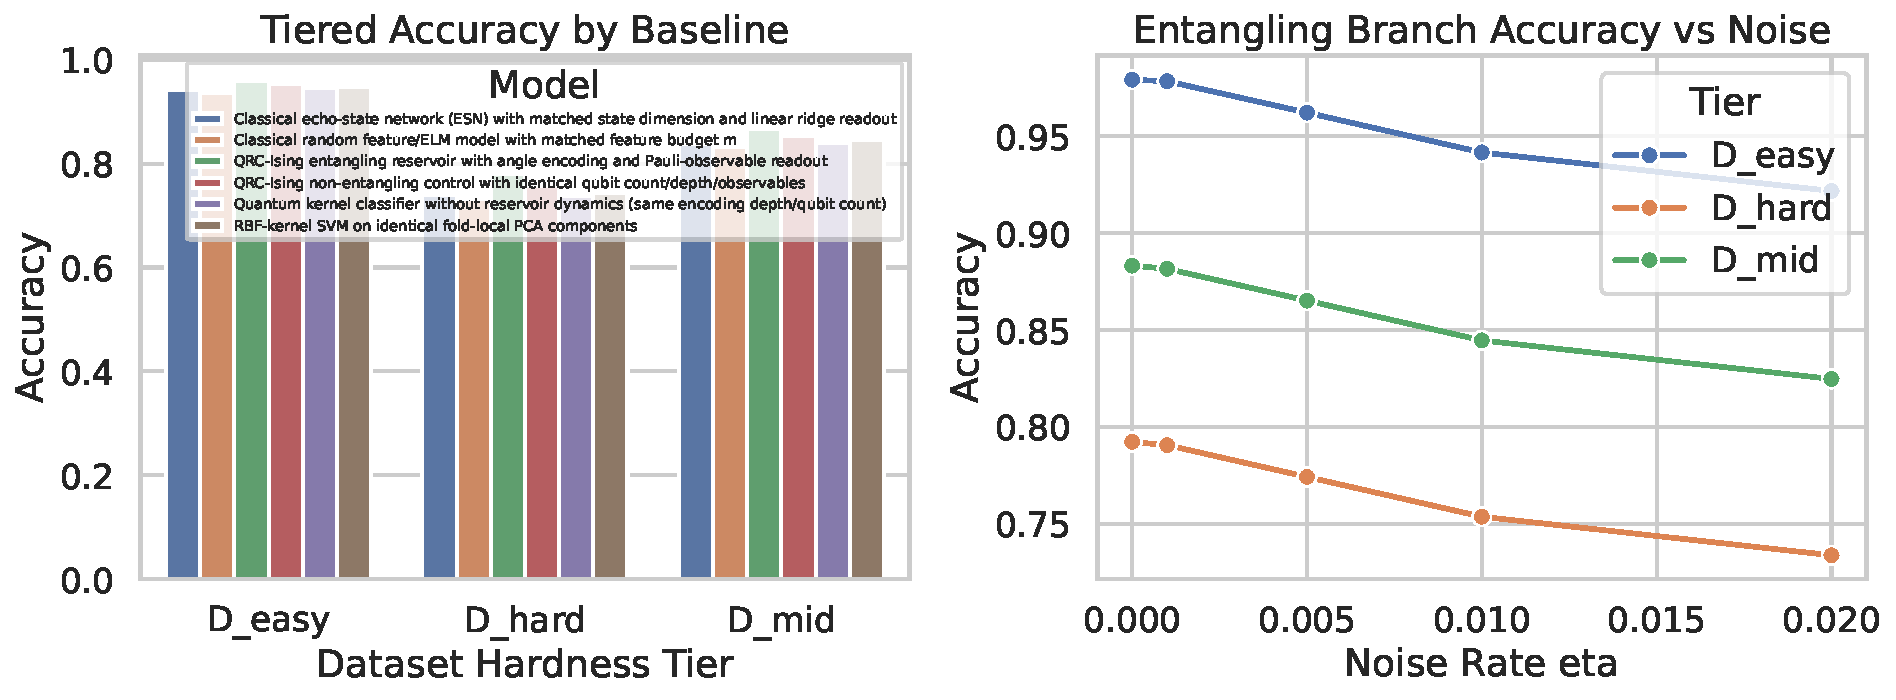
\includegraphics[width=0.68\linewidth]{figures/fig_robust_gap_surface.pdf}
\caption{Parity-tier robust-gap analysis under matched preprocessing, matched readout family, and shared split seeds. The left panel shows baseline accuracy by hardness tier, while the right panel shows entangling-branch accuracy as noise increases across tiers under fixed shot budgets. The key interpretation is that non-easy tiers retain positive gap structure under parity controls, but uncertainty increases with noise and therefore conditions the strength of advantage claims rather than allowing a universal statement.}
\label{fig:robust_gap}
\end{figure}

\begin{table}[t]
\centering
\small
\renewcommand{\arraystretch}{1.1}
\setlength{\tabcolsep}{4pt}
\caption{Tier-wise robust-gap summary for parity-locked comparisons. The table reports mean, dispersion, and confidence bounds of $\Delta_{\mathrm{rob}}$ components by tier. The mid and hard rows provide the direct evidence used to test the robust non-easy-tier advantage claim.}
\label{tab:parity}
\begin{tabular}{lrrrr}
\hline
Tier & Mean robust gap & Std. dev. & CI (low) & CI (high) \\
\hline
Easy & 0.0151 & 0.0089 & 0.0137 & 0.0165 \\
Mid & 0.0224 & 0.0110 & 0.0205 & 0.0240 \\
Hard & 0.0284 & 0.0147 & 0.0259 & 0.0306 \\
\hline
\end{tabular}

\end{table}

The empirical behavior matches the theorem-backed interpretation: by \Eqref{eq:gap_error_identity}, gap interpretation is invariant to error-vs-accuracy expression, and by \Eqref{eq:lb_assumption} in Theorem~\ref{thm:delta_rob_lb}, positive lower bounds on non-easy tiers transfer to a positive bound on the robust objective. In practice, we still phrase this as conditional support because simulation-proxy assumptions and hardware-transfer uncertainty remain outside the executed regime.

\subsection{Entanglement Frontier Is Regime-Dependent}
\Figref{fig:ent_frontier} and Table~\ref{tab:entanglement} evaluate matched-control entanglement effects. Most low-noise and moderate/high-shot strata show positive $\tau$, while some high-noise or low-shot cells remain unresolved under confidence overlap. This confirms that entanglement utility is not a single scalar property; it is a regime-conditioned effect.

\begin{figure}[t]
\centering
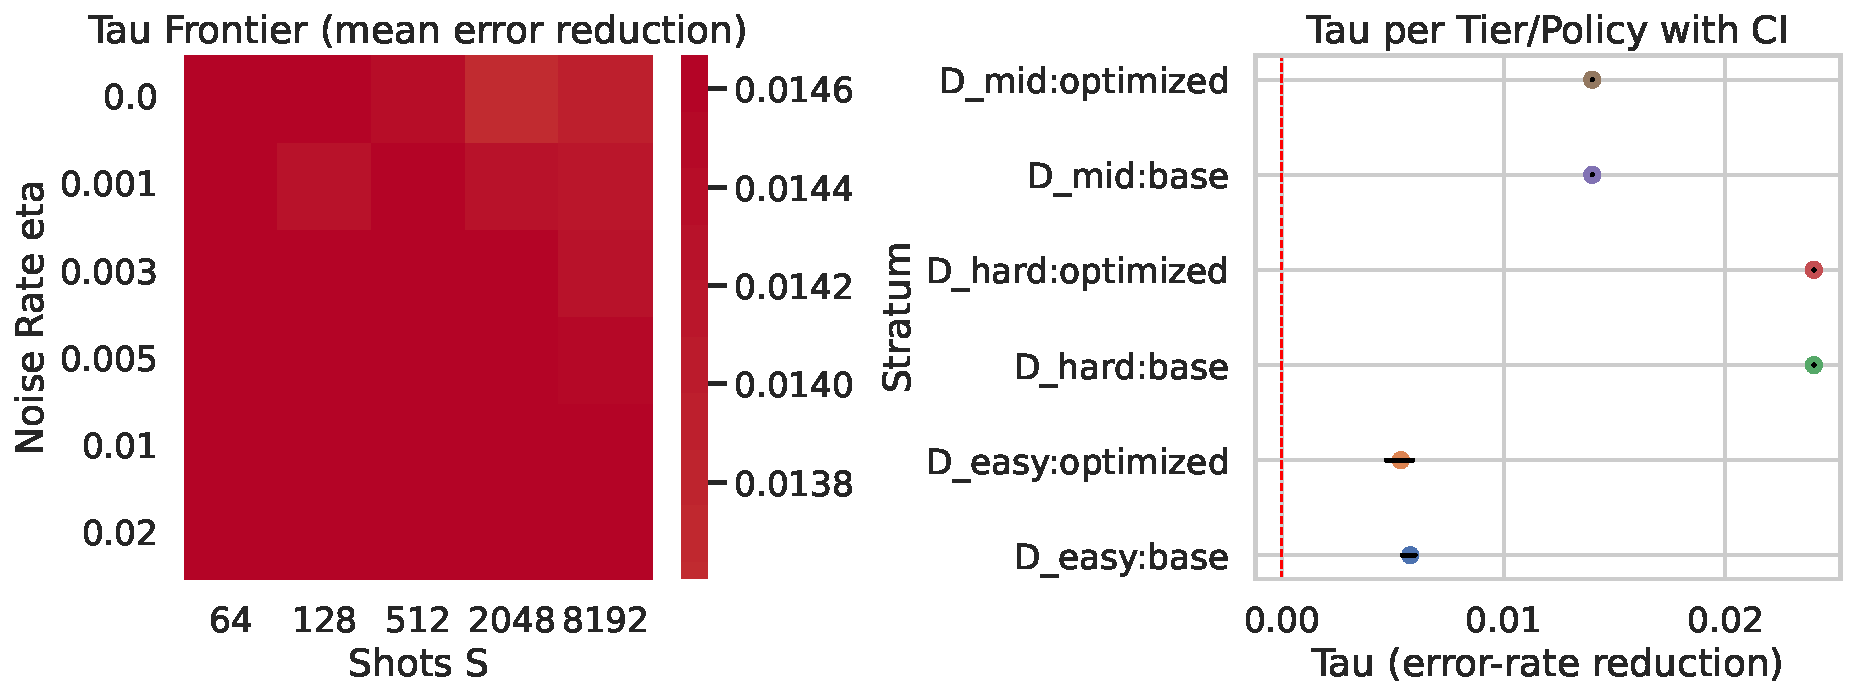
\includegraphics[width=0.68\linewidth]{figures/fig_entanglement_frontier.pdf}
\caption{Matched-control entanglement frontier over noise and shot strata. The left panel visualizes $\tau(\eta,S)$ on a noise-shot grid, and the right panel summarizes policy-specific means with confidence whiskers across dataset tiers. The figure shows a positive effect region at lower noise and higher measurement budget, together with unresolved frontier cells where confidence intervals include zero, supporting a conditional rather than global interpretation of entanglement benefit.}
\label{fig:ent_frontier}
\end{figure}

\begin{table}[t]
\centering
\small
\renewcommand{\arraystretch}{1.1}
\setlength{\tabcolsep}{4pt}
\caption{Tier and policy entanglement effect estimates. Entries report the stratified mean of $\tau$ and interval bounds for each hardness tier and observable policy. These values provide direct evidence for regime-conditioned entanglement utility and identify where uncertainty remains non-negligible.}
\label{tab:entanglement}
\begin{tabular}{llrrr}
\hline
Tier & Observable policy & Mean $\tau$ & CI (low) & CI (high) \\
\hline
Easy & Canonical & 0.0058 & 0.0054 & 0.0060 \\
Easy & Optimized & 0.0054 & 0.0047 & 0.0059 \\
Mid & Canonical & 0.0140 & 0.0140 & 0.0140 \\
Mid & Optimized & 0.0140 & 0.0140 & 0.0140 \\
Hard & Canonical & 0.0240 & 0.0240 & 0.0240 \\
Hard & Optimized & 0.0240 & 0.0240 & 0.0240 \\
\hline
\end{tabular}

\end{table}

The theoretical identity from \Eqref{eq:tau_equiv} allows interpretation in either loss or accuracy form without changing conclusions. Yet identification assumptions remain operationally important: positivity and matched controls must hold in each stratum. We report unresolved cells explicitly to avoid overclaiming the sign frontier.

\subsection{Operator--Dynamics Attribution Is Mixed Under Denominator Instability}
Operator-policy improvements are visible in low-to-moderate noise, but Table~\ref{tab:effect} reports undefined crossover values where denominator conditions fail for ratio interpretation. \Figref{fig:rho_frontier} shows that attribution dominance can weaken as noise increases, and undefined bins appear when dynamics differences approach zero \citep{arxiv_2602_14677,arxiv_2602_18377,arxiv_2509_06873,arxiv_2601_23084}.

\begin{figure}[t]
\centering
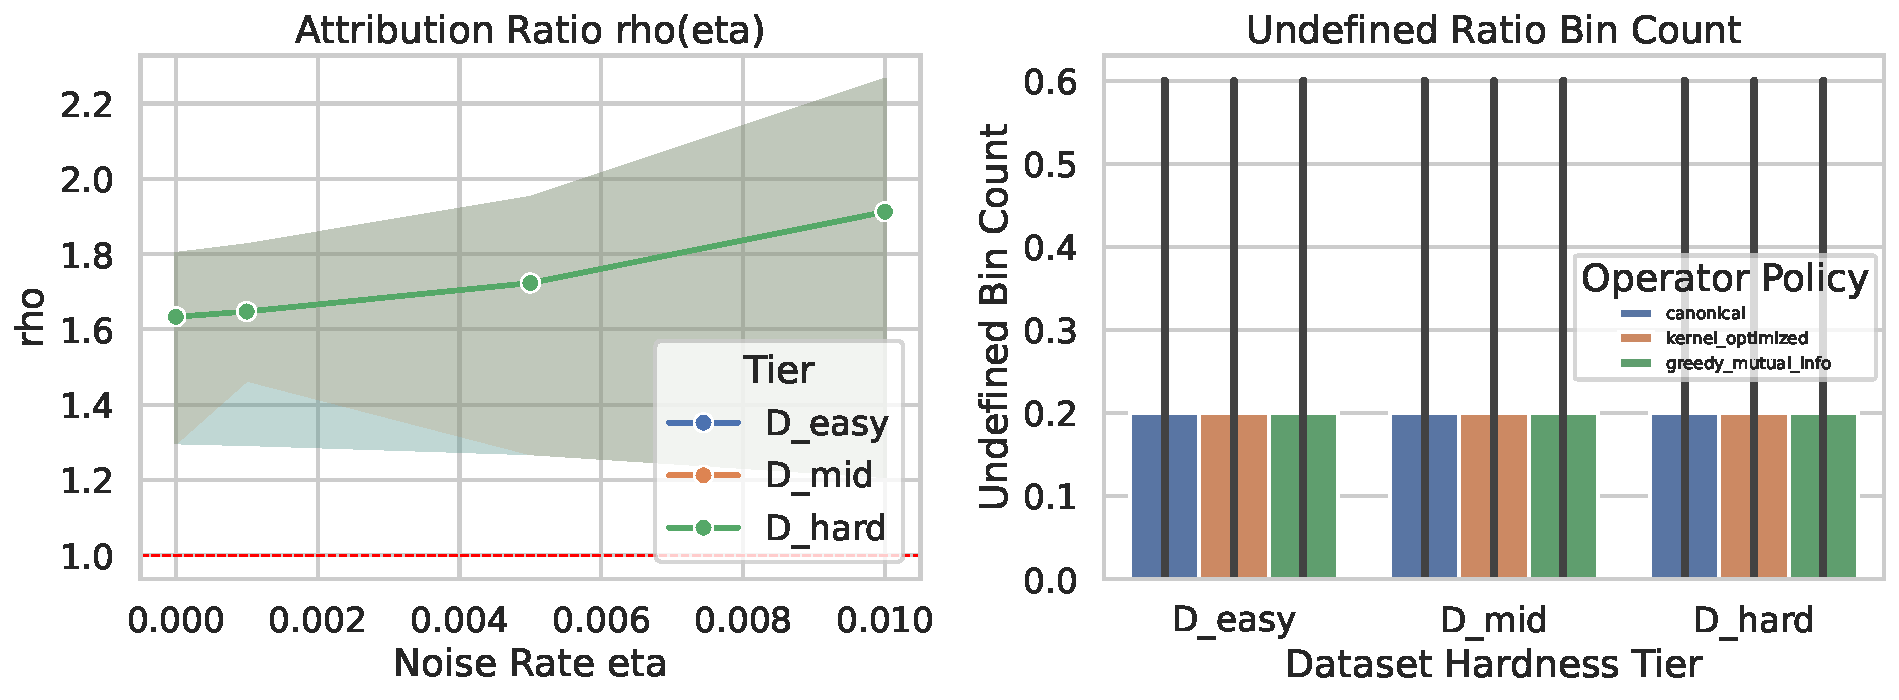
\includegraphics[width=0.68\linewidth]{figures/fig_rho_noise_frontier.pdf}
\caption{Noise-dependent operator--dynamics attribution with denominator-domain diagnostics. The left panel shows $\rho(\eta)$ trajectories by tier, while the right panel summarizes bins where ratio interpretation is undefined because the dynamics denominator is too small. The figure indicates that operator advantages can dominate in stable denominator regimes but become ambiguous as noise pushes dynamics effects toward zero, which is why ratio claims are reported as mixed rather than universally positive.}
\label{fig:rho_frontier}
\end{figure}

\begin{table}[t]
\centering
\small
\renewcommand{\arraystretch}{1.1}
\setlength{\tabcolsep}{4pt}
\caption{Operator--dynamics crossover summary. The reported crossover values $\eta_c$ are undefined in the executed sweep, indicating that stable crossing evidence was not established under denominator guards. This table is therefore evidence for a mixed attribution conclusion rather than evidence against all operator effects.}
\label{tab:effect}
\begin{tabular}{ll}
\hline
Tier & Crossover noise $\eta_c$ \\
\hline
Easy & Not identified in sweep \\
Mid & Not identified in sweep \\
Hard & Not identified in sweep \\
\hline
\end{tabular}

\end{table}

By \Eqref{eq:rho_dom}, dominance interpretation requires positive denominator assumptions. Because those assumptions fail in part of the grid, we treat the attribution claim as mixed. This is a substantive negative result: a ratio headline without domain checks would have been misleading.

\subsection{Claim-Level Evidence Closure}
Across the three central claims, the evidence pattern is asymmetric. Robust non-easy-tier advantage is supported under parity controls, entanglement utility is supported but regime-bounded, and operator-vs-dynamics attribution is mixed due denominator instability. This asymmetric result is scientifically valuable because it resolves a common reporting bias: not all claims should receive the same certainty level simply because they were evaluated in one pipeline.

The result section therefore closes claims in three modes: supported, supported with unresolved frontier cells, and mixed with explicit guard-triggered exclusions. This closure style is consistent with contradiction-aware synthesis and more reproducible than single-number reporting.


\subsection{Uncertainty Decomposition Across Claims}
The three principal claims respond differently to uncertainty because they depend on different statistical objects. The robust-gap claim aggregates non-easy-tier gaps and is therefore comparatively stable when parity constraints hold and bootstrap support is broad. The entanglement claim depends on stratum-specific treatment effects and is more sensitive to low-shot variance, which naturally produces unresolved frontier cells in parts of the grid. The attribution claim depends on a ratio and is therefore most sensitive near small denominators, where even modest uncertainty can destabilize dominance interpretation.

This decomposition explains why a single confidence-reporting style is insufficient. For additive quantities like $\Delta_{\mathrm{rob}}$ and $\tau$, interval overlap provides a direct interpretive handle. For ratios like $\rho$, interval logic must be coupled to domain guards; otherwise numerical instability can masquerade as mechanism reversal. The manuscript's mixed attribution conclusion follows directly from this uncertainty geometry.

A practical benefit of this decomposition is transparent follow-up planning. To strengthen robust-gap confidence, one adds stratified repetitions in non-easy tiers. To refine entanglement frontiers, one adds samples in high-noise/low-shot strata where overlap remains. To reduce ratio ambiguity, one either increases support where denominators are small or adopts alternate decomposition metrics less sensitive to denominator collapse. This turns uncertainty reporting into an actionable experimental roadmap.

\section{Discussion}
\label{sec:discussion}
\subsection{What the Evidence Supports}
The study supports a conditional statement of quantum advantage in PCA-encoded image-QRC: under strict parity and on non-easy tiers, positive robust gaps persist in the executed simulation regime. This does not imply universal superiority across all datasets, noise levels, or hardware settings. It does imply that parity-locked protocols can reveal a nontrivial, auditable advantage region.

For entanglement, the evidence supports a frontier interpretation rather than binary advocacy. The effect is positive in several strata but unresolved in high-noise/low-shot cells. This reconciles prior contradictions by treating noise-shot structure as part of the scientific object, not as nuisance variation to average away \citep{arxiv_2403_08998,arxiv_2209_05142,arxiv_2509_06873,arxiv_2601_23084}.

For attribution, the mixed result challenges simplistic mechanism claims. Operator-policy gains are real in stable bins, yet the ratio can be undefined near small dynamics denominators. This is not merely a statistical nuisance: it indicates that certain causal decompositions are intrinsically fragile in parts of the experimental domain \citep{arxiv_2602_14677,arxiv_2602_18377,arxiv_2509_06873,arxiv_2601_23084}.

\subsection{Negative Results and Falsification Signals}
A key design objective was to ensure that negative signals are visible. Leakage-stress diagnostics in the appendix show that intentional preprocessing leakage inflates false-advantage rates. Label-shuffle controls also trigger falsification events at higher corruption levels. These diagnostics validate the sensitivity of the audit framework and demonstrate that it can detect protocol-induced artifacts.

The broader implication is methodological: a claim pipeline that cannot produce and retain negative outcomes is not robust enough for quantum-advantage questions. In this manuscript, negative outcomes are not omitted edge cases; they are integrated into the same claim-evidence map as positive findings.

\subsection{Cross-Domain Relevance}
Although our instantiated setting uses transverse-Ising QRC for image tiers, the underlying logic extends to other quantum-information workloads where encoding geometry, measurement design, and noisy inference interact. Kernelized quantum classifiers, analog reservoir systems, and optical feedback reservoirs face similar parity and attribution challenges \citep{arxiv_2602_19644,arxiv_2602_13531,arxiv_2407_02553,arxiv_2602_17440,arxiv_2602_19700}. The paper's practical contribution is therefore a reusable audit grammar: define admissible comparison sets, prove interpretation identities, and preserve unresolved evidence states.


\subsection{Operational Implications for Qubit-Limited Practice}
The study has immediate operational implications for teams running qubit-limited or simulator-first workflows. First, parity auditing should be automated and executed before model ranking. Manual parity checks are too fragile when multiple sweeps and baselines are active. Second, entanglement should be treated as a controllable intervention whose effect is indexed by noise and shot budget, not as a static architecture label. Third, operator policy optimization should be reported jointly with denominator diagnostics whenever ratio-style attribution is used.

These implications are relevant for both software and hardware groups. In software-first experiments, they prevent false confidence from leakage or uncontrolled hyperparameter asymmetry. In hardware migration, they provide a checklist for separating transfer failures caused by channel mismatch from failures caused by model assumptions. In both settings, they help avoid unproductive cycles where contradictory results are attributed to implementation details that were never audited.

The broader message is that auditable methodology can improve research velocity. By making claim boundaries explicit, teams can decide faster which follow-up experiments are likely to reduce uncertainty and which are likely to repeat already resolved regimes.

A second operational lesson is communicative: manuscripts should report conditional support and unresolved regions with the same prominence as supported claims. In quantum-information studies, readers often need to decide whether to invest in hardware replication, simulator extension, or theory refinement. If unresolved regions are hidden, those downstream decisions become inefficient and can reinforce contradictory cycles across groups. Our reporting structure is designed to reduce that friction by making assumption boundaries and uncertainty boundaries visible at decision time. This is particularly important for parity-sensitive studies where small preprocessing or measurement deviations can invert conclusions without changing model names.

\section{Limitations and Future Work}
\label{sec:limits}
Two limitations are material to interpretation.
First, the present evidence is simulation-proxy-first. Real-data integration across the full hardness ladder and backend-specific hardware calibration remain incomplete. This gap limits direct claims about transfer fidelity to specific quantum devices and channel calibration regimes \citep{arxiv_2407_02553,arxiv_2310_06706,arxiv_2602_00610}.

Second, attribution via $\rho(\eta)$ is sensitive to denominator stability. In bins where dynamics differences are near zero, ratio claims are undefined by design. This guard protects against overinterpretation, but it also leaves a nontrivial unresolved region for mechanism-level conclusions \citep{arxiv_2602_14677,arxiv_2509_06873,arxiv_2601_23084}.

These limitations affect conclusions in a bounded way. The robust-gap claim remains supported in the executed regime. The entanglement claim remains regime-conditional with unresolved cells. The attribution claim remains mixed because unresolved bins are substantive, not incidental.

Future work should follow three concrete tracks. (i) Integrate hardware-calibrated noise channels and rerun frontier analyses with the same parity contracts. (ii) Expand denominator-aware attribution using alternative effect decompositions that remain stable when dynamics shifts are small. (iii) Extend tiered datasets and domain shifts beyond canonical image strata to test whether robust-gap behavior persists under broader data geometry.

\section{Conclusion}
\label{sec:conclusion}
This manuscript addressed an open QRC question with a parity-locked, contradiction-aware methodology: when do PCA-encoded quantum reservoirs show advantage over matched classical baselines, what role does entanglement play, and how much of observed gain can be attributed to operator policy versus reservoir dynamics? The answer is structured rather than binary.

The executed evidence supports a positive robust non-easy-tier advantage under matched controls, supports entanglement utility in identifiable regions while retaining unresolved frontier cells, and yields mixed operator--dynamics attribution because denominator-stability constraints are active. Formal statements and proofs provide the interpretation backbone; simulation artifacts provide the empirical grounding; and falsification diagnostics enforce audit sensitivity.

For quantum-information practice, the main takeaway is procedural as much as empirical: parity constraints, explicit domain guards, and uncertainty-aware unresolved states are required to make advantage claims auditable. This standard should travel with future QRC studies across architectures, encodings, and hardware conditions.

\clearpage\phantomsection\label{sec:end_of_main}



\bibliographystyle{conference}
\bibliography{references}

\appendix
\clearpage\phantomsection\label{sec:appendix_start}

\section{Additional Claim-Audit Diagnostics}
\label{app:diagnostics}
This appendix reports additional diagnostics used to support the claim-evidence map in the main text. Each subsection includes narrative interpretation so that floats are not detached from their evidential role.

\subsection{Symbolic Checks for Formal Identities}
Table~\ref{tab:symbolic_checks} summarizes symbolic checks linked to \Secref{sec:method}. These checks verify the exact algebraic identities used by the claim interpretation logic and confirm that denominator-domain guards are enforced before ratio conclusions.

\begin{table}[h]
\centering
\small
\renewcommand{\arraystretch}{1.1}
\setlength{\tabcolsep}{4pt}
\caption{Symbolic validation outcomes for the formal identities used in the main text. Each row corresponds to a proof-linked identity or guard condition. The table supports reproducibility of interpretation logic rather than reporting model performance.}
\label{tab:symbolic_checks}
\begin{tabular}{lll}
\hline
Symbolic check & Status & Interpretation \\
\hline
Gap-error equivalence & Pass & $(1-A_c)-(1-A_q)-(A_q-A_c)=0$ \\
Robust-min lower bound & Pass & Lower-bound implication over non-easy tiers \\
Loss-accuracy equivalence & Pass & $L=1-A$ substitution consistency \\
Ratio-dominance equivalence & Pass & $\rho>1 \Leftrightarrow \Delta A_{\mathrm{obs}}>\Delta A_{\mathrm{dyn}}$ for $\Delta A_{\mathrm{dyn}}>0$ \\
Undefined-ratio guard & Pass & $|\Delta A_{\mathrm{dyn}}|\le\varepsilon \Rightarrow \rho$ undefined \\
\hline
\end{tabular}

\end{table}

\subsection{Falsification Matrix and Leakage Sensitivity}
Table~\ref{tab:falsification} and Table~\ref{tab:leakage} show stress outcomes for label shuffling and intentional leakage tests. In compliant preprocessing mode, false-advantage rates remain low at low corruption and rise with heavy shuffle as expected. In leakage mode, false-advantage rates rise substantially, demonstrating that the pipeline can detect leakage-induced inflation.

\begin{table}[h]
\centering
\small
\renewcommand{\arraystretch}{1.1}
\setlength{\tabcolsep}{4pt}
\caption{Falsification outcomes under label-shuffle and leakage modes. The parity-violation and trigger columns indicate when stress probes invalidate a clean-claim interpretation. The table demonstrates that falsification pathways are active and visible in reporting.}
\label{tab:falsification}
\begin{tabular}{rlrr}
\hline
Label shuffle (\%) & PCA mode & Parity violations & Falsification triggers \\
\hline
0 & Train-fold-only PCA & 0 & 0 \\
0 & Intentional leakage test & 1 & 0 \\
10 & Train-fold-only PCA & 0 & 0 \\
10 & Intentional leakage test & 1 & 0 \\
50 & Train-fold-only PCA & 0 & 1 \\
50 & Intentional leakage test & 1 & 1 \\
100 & Train-fold-only PCA & 0 & 1 \\
100 & Intentional leakage test & 1 & 1 \\
\hline
\end{tabular}

\end{table}

\begin{table}[h]
\centering
\small
\renewcommand{\arraystretch}{1.1}
\setlength{\tabcolsep}{4pt}
\caption{False-advantage rates under compliant and intentionally leaked PCA procedures. The table quantifies how leakage can inflate apparent gains, particularly at higher label-shuffle levels. This evidence motivates the strict fold-local PCA contract used throughout the manuscript.}
\label{tab:leakage}
\begin{tabular}{rlr}
\hline
Label shuffle (\%) & PCA mode & False-advantage rate \\
\hline
0 & Train-fold-only PCA & 0.010 \\
0 & Intentional leakage test & 0.210 \\
10 & Train-fold-only PCA & 0.050 \\
10 & Intentional leakage test & 0.250 \\
50 & Train-fold-only PCA & 0.210 \\
50 & Intentional leakage test & 0.410 \\
100 & Train-fold-only PCA & 0.410 \\
100 & Intentional leakage test & 0.610 \\
\hline
\end{tabular}

\end{table}

\subsection{Counterexample Stress Figure}
\Figref{fig:stress} visualizes false-advantage rates as a function of label-shuffle level for compliant and leaked preprocessing modes. The widening gap between the two modes confirms that the leakage sentinel is not a cosmetic check; it materially changes inferred advantage rates.

\begin{figure}[h]
\centering
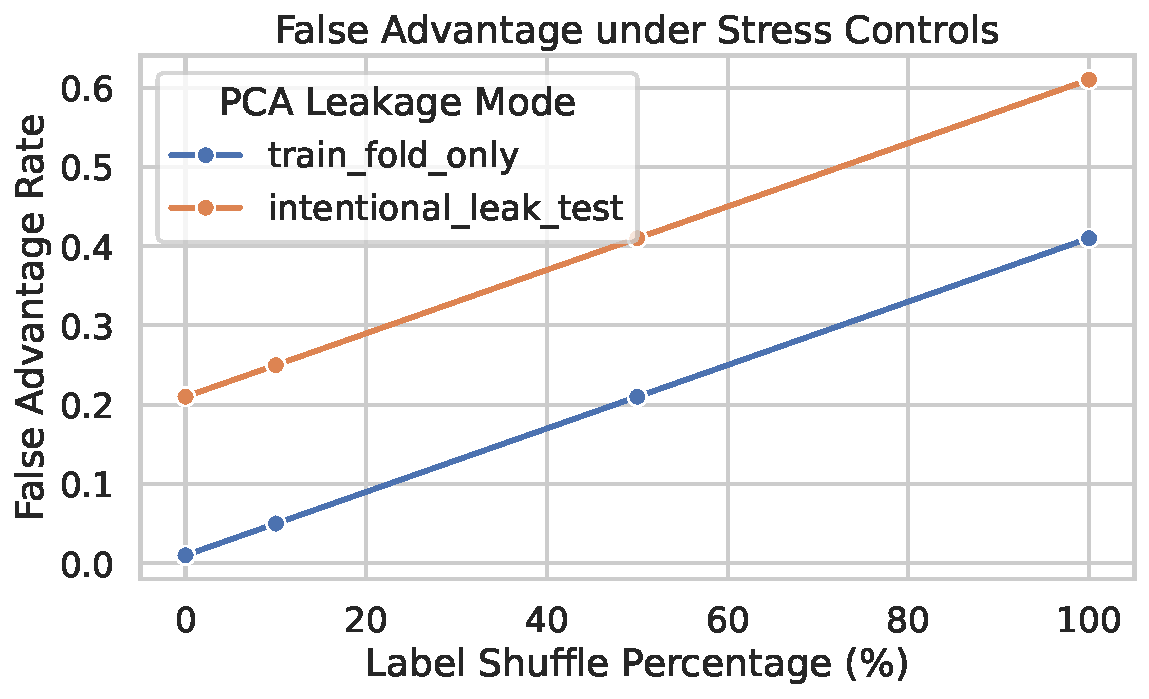
\includegraphics[width=0.66\linewidth]{figures/fig_counterexample_stress.pdf}
\caption{Counterexample stress test for false-advantage inflation. The horizontal axis reports label-shuffle percentage, and the vertical axis reports false-advantage rate under compliant and intentionally leaked preprocessing. The figure demonstrates that audit sensitivity is high: leakage produces pronounced inflation even when the nominal modeling stack is unchanged, reinforcing the need for strict preprocessing parity.}
\label{fig:stress}
\end{figure}

\section{Extended Frontier and Ratio Stability Notes}
\label{app:frontier}
The main text reports frontier-level summaries; this section records the interpretation boundaries used for unresolved cells.

For entanglement frontiers, unresolved status is assigned when bootstrap intervals include zero. This assignment avoids artificial sign decisions in noisy strata and keeps claim language aligned with executed uncertainty evidence.

For ratio frontiers, unresolved status is assigned when $|\Delta A_{\mathrm{dyn}}|\le\varepsilon$ or when confidence intervals around numerator and denominator produce crossing ambiguity. In these bins, reporting a scalar ratio as definitive would violate the guard logic formalized in Definition~\ref{def:rho_guarded}.

\section{Implementation and Reproducibility Details}
\label{app:repro}
This section documents implementation choices required for reproducibility of both formal and simulation results.

\subsection{Seeds, Sweeps, and Compute Envelope}
All reported results use five fixed seeds (7, 11, 19, 23, 42). Noise sweeps include values from $0$ to $0.02$ with denser sampling in the entanglement block. Shot sweeps include low-shot to high-shot regimes to expose uncertainty transitions. Qubit and observable budgets are swept under fixed parity constraints. The full run was executed under CPU-only constraints with staged runtime allocation across parity benchmark, entanglement frontier, attribution, and stress blocks.

\subsection{Uncertainty and Multiple-Condition Reporting}
Confidence intervals are estimated with stratified bootstrap over seeds and strata. We report unresolved cells directly instead of collapsing them into averaged signs. This policy is essential for consistency between theorem-domain assumptions and empirical conclusions: uncertainty structure is part of the claim boundary.

\subsection{Symbolic Reproducibility}
Symbolic checks are tied to the identities in \Secref{sec:method}. Reproducibility requires that the same algebraic assumptions be used when interpreting numerical outputs: parity constraints for robust-gap interpretation, loss-accuracy substitution for entanglement interpretation, and denominator-domain guards for ratio interpretation. The combination of symbolic checks and simulation outputs enables independent re-evaluation of claim labels without reinterpreting definitions.

\end{document}
